%%%%%%%%%%%%%%%%%%%%%%%%%%%%%%%%%%%%%%%%%%%%%%%%%%%%%%%%%%%%%%%%%%%%%%%%
\chapter{Introduction}
\label{chapter:introduction}
%%%%%%%%%%%%%%%%%%%%%%%%%%%%%%%%%%%%%%%%%%%%%%%%%%%%%%%%%%%%%%%%%%%%%%%%
\localtableofcontents

% \section{Context}
%
% Neural networks are now present all around us and in all areas.
% Without knowing it, an average person uses them every day; automatic translators, chatbots, voice assistants, recommendations, etc.
% The applications are very diverse and can have a profound impact on entire sectors (transport, health care, etc.).
% If the use of neural networks is so important, it is because they are so effective in \emph{learning} any type of task with results that are close to perfection, surpassing man on many points.
%
% However, although widely in use, Neural Networks are not perfect, a lot of open questions remain and many problems have emerged.
% This thesis attempts to highlight and answer some of the problems that Neural Networks face.

% %%%%%%%%%%%%%%%%%%%%%%%%%%%%%%%%%%%%%%%%%%%%%%%%%%%%%%%%%%%%%%%%%%%%%%%%%%%%%%%
% \section{Introduction to Supervised Learning \& Neural Networks}
% \label{section:ch1-introduction_to_supervised_learning_and_neural_networks}
% %%%%%%%%%%%%%%%%%%%%%%%%%%%%%%%%%%%%%%%%%%%%%%%%%%%%%%%%%%%%%%%%%%%%%%%%%%%%%%%
%
% In recent years, with the advent of data collection, \emph{supervised learning} have shown great success in different domain such as computer vision~\cite{xxx, xxx, xxx}, natural language processing~\cite{xxx, xxx}, speech recognition~\cite{hinton2012deep}.  visionobject recognition in computer vision~\cite{xxx}, spam detection~\cite{xxx}, recommendation~\cite{xxx}
%
%
% natural language processing~\cite{radford2018Language}, image recognition~\cite{He_2016_CVPR} and speech recognition~\cite{hinton2012deep}.
% Machine Learning algorithms consists of learning a function which performs a certain task from sample data. 
%
% \emph{Supervised Learning algorithms}, which are a subset of Machine Learning algorithms, consist of learning the relation between the data and its label. 
%
% The process of \emph{training} consists of several steps: first, a function parameterized by weights is randomly initialized. Then, the algorithm will \emph{analyzed} the data and \emph{adjust} the weights iterativly until 
%


%%%%%%%%%%%%%%%%%%%%%%%%%%%%%%%%%%%%%%%%%%%%%%%%%%%%%%%%%%%%%%%%%%%%%%%%%%%%%%%
\section{Introduction to Supervised Learning and Neural Networks}
\label{secction:ch2-supervised_learning_neural_networks}
%%%%%%%%%%%%%%%%%%%%%%%%%%%%%%%%%%%%%%%%%%%%%%%%%%%%%%%%%%%%%%%%%%%%%%%%%%%%%%%


%%%%%%%%%%%%%%%%%%%%%%%%%%%%%%%%%%%%%%%%%%%%%%%%%%%%%%%%%%%%%%%%%%%%%%%%%%%%%%%
\subsection{Introduction to Supervised Learning}
\label{subsection:ch1-introduction_to_supervised_learning}
%%%%%%%%%%%%%%%%%%%%%%%%%%%%%%%%%%%%%%%%%%%%%%%%%%%%%%%%%%%%%%%%%%%%%%%%%%%%%%%

This thesis focus on the concept of \emph{supervised learning} which refers to the notion of learning the parameters of a specific function that maps an input to an output based on example input-output pairs.
For example, an image (input) associated with its content: label (output).
% The choice of the function used for supervised learning is an active area of research and will be part of the focus of this thesis.

Let us consider an input space $\mathcal{X} = [0, 1]^d$ of dimension $d$, an output space $\mathcal{Y} = [k]$ where $k$ is the number of classes and a data distribution $\mathcal{D}$ over $\mathcal{X} \times \mathcal{Y}$.
In supervised learning, we seek to find a function $h: \mathcal{X} \rightarrow \mathcal{Y}$ that maps the input $\xvec \in \mathcal{X}$ to the output $y \in \mathcal{Y}$ with $h \in \mathcal{H}$ where $h$ is called the \emph{hypothesis} and $\mathcal{H}$ the \emph{hypothesis space}.
In order to measure how well the function fits, a \emph{loss function} $L: \mathcal{Y} \times \mathcal{Y} \rightarrow \Rbb^{+}$ is defined.
The \emph{risk} $R$ associated with the hypothesis $h(\xvec)$ is defined as follows:
\begin{equation}
  R(h) \triangleq \Ebb_{(\xvec, y) \sim \mathcal{D}}\  L \left( h(\xvec), y \right)
\end{equation}
The goal of a \emph{learning algorithm} is to find a hypothesis $h^* \in \mathcal{H}$ which minimizes the risk $R(h)$:
\begin{equation}
  h^* \triangleq \argmin_{h \in \mathcal{H}} R(h) .
\end{equation}

% \paragraph{Empirical Risk Minimization} (ERM).
In practice, the joint probability distribution $\mathcal{D}$ is unknown.
Instead, we have $n$ independent observations of the distribution called the \emph{training set}
\begin{equation}
  \left\{ (\xvec^{(1)}, y^{(1)} ), \dots, ( \xvec^{(n)}, y^{(n)} ) \right\} ,
\end{equation}
where $\xvec \in \mathcal{X}$ and $y \in \mathcal{Y}$.
The risk minimization problem is therefore replaced by the \emph{empirical risk minimization} (ERM) as follows:
\begin{equation}
  E(h, n) \triangleq \frac{1}{n} \sum_{i = 1}^{n} L\left(h(\xvec^{(i)}), y^{(i)}\right) ,
\end{equation}
the learning algorithm then becomes:
\begin{equation}
  \hat{h}^* \triangleq \argmin_{h \in \mathcal{H}} E(h, n)  .
\end{equation}

In this thesis, we will use and study \emph{neural networks} which are a class of function commonly used for unstructured datasets (image, sound, text).


%%%%%%%%%%%%%%%%%%%%%%%%%%%%%%%%%%%%%%%%%%%%%%%%%%%%%%%%%%%%%%%%%%%%%%%%%%%%%%%
\subsection{Introduction to Neural Networks}
\label{subsection:ch1-introduction_to_neural_networks}
%%%%%%%%%%%%%%%%%%%%%%%%%%%%%%%%%%%%%%%%%%%%%%%%%%%%%%%%%%%%%%%%%%%%%%%%%%%%%%%

Neural Networks find their roots, in 1958, in the works of Frank Rosenblatt \cite{rosenblatt1958perceptron} where for the first time, the Perceptron, an electronic device inspired by the human brain, showed ability to \emph{learn} from multiple examples.
In essence, the Perceptron is an algorithm for learning a binary classifier, this classifier can be analytically described as a composition of a linear function $\phi$ and the Heaviside step function $\rho$ as follows:
\begin{equation}
  f(\xvec) = \rho \circ \phi(\xvec) = \left\{ 
    \begin{aligned}
      &1 \quad \text{if} \quad \phi(\xvec) > 0  \\
      &0 \quad \text{otherwise}
    \end{aligned}
    \right. .
\end{equation}
where $\phi(\xvec) = \wvec^\top \xvec$ is a linear function and the values of the vector $\wvec$ are the learned parameters. 
However, a few years after its introduction, \citet{minsky1969perceptrons} demonstrated important limitations of the Perceptron.
Indeed, although theoretically capable of classifying any linear separable problem, it is not able to correctly classify simple non-linear functions (see Figure~\ref{figure:xor_function}).
\begin{figure}[htb]
  \centering
  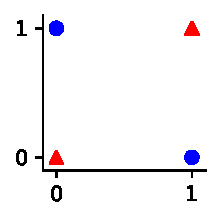
\includegraphics{figures/chapter1/xor_function.pdf}
  \caption{Graphical representation of the XOR function. This function cannot be separated by a linear classifier.}
  \label{figure:xor_function}
\end{figure}
To circumvent these limitations, \citet{minsky1969perceptrons} considered that \emph{another layer of logic} could be added to the function allowing the classification to be done on another representation (see Figure~\ref{figure:multi_layer_perceptron}).
Let $\phi_1$ and $\phi_2$ be two linear functions, we could define a \emph{Multi-Layer Perceptron} as follows:
\begin{equation}
  f(\xvec) = \rho \circ \phi_2 \circ \rho \circ \phi_1( \xvec )
\end{equation}

\begin{figure}[ht]
  \centering
  \begin{subfigure}[t]{0.30\textwidth}
    \centering
    \begin{tabular}{c|c}
      \multicolumn{2}{c}{$\xvec$} \\
      \midrule
      0 & 0 \\
      0 & 1 \\
      1 & 0 \\
      1 & 1
    \end{tabular} 
    \caption*{Input representation}
  \end{subfigure}
  \begin{subfigure}[t]{0.03\textwidth}
    $\rightarrow$
  \end{subfigure}
  \begin{subfigure}[t]{0.30\textwidth}
    \centering
    \begin{tabular}{C{0.5cm} | C{0.5cm}}
      \multicolumn{2}{c}{$\rho \circ \phi_1(\xvec)$} \\
      \midrule
      0 & 0 \\
      0 & 1 \\
      1 & 0 \\
      0 & 0
    \end{tabular}
    \caption*{Intermediate representation}
  \end{subfigure}
  \begin{subfigure}[t]{0.03\textwidth}
    $\rightarrow$
  \end{subfigure}
  \begin{subfigure}[t]{0.30\textwidth}
    \centering
    \begin{tabular}{c}
      $f(\xvec)$ \\
      \midrule
      0 \\
      1 \\
      1 \\
      0
    \end{tabular}
    \caption*{Final representation}
  \end{subfigure}
  \caption{Classification of the XOR function with a Multi-Layer Perceptron}
  \label{figure:multi_layer_perceptron}
\end{figure}

One of the first \emph{Multi-Layer Perceptron}, or now more commonly known as \emph{Deep Neural Network}, was introduced by~\citeauthor{ivakhnenko1967cybernetics} in~\citeyear{ivakhnenko1967cybernetics}.
More precisely, a Neural Neural can be analytically described as a composition of linear functions interlaced with non-linear functions (also called activation functions):
\begin{equation}
  f_\Theta(\xvec) = \phi_{\Wmat_p} \circ \rho \circ \phi_{\Wmat_{p-1}} \circ \cdots \circ \phi_{\Wmat_2} \circ \rho \circ \phi_{\Wmat_1}(\xvec)
  \label{equation:neural_network}
\end{equation}
where the function $\phi_{\Wmat_i}$ is a linear function parameterized by $\Wmat_i$, $\rho$ is a non-linear function, $\Theta \triangleq ( \Wmat_1, \dots, \Wmat_p )$ and $p$ correspond to the \emph{depth} of the network (\ie, the number of layers).
If the weight matrices are dense, this architecture is called \emph{Fully Connected Neural Network} because all the neurons from the first activation are connected to all the neurons from the second activation.

Therefore, a neural network is a function $f_\Theta:\Rbb^n \rightarrow \Rbb^m$ parameterized by weights and composed of at least two linear functions (layers) and one non-linear function (activation function).
The input space $n$ is usually large and the output space $m$ corresponds to the number of classes the network has to classify; therefore, we have $m \ll n$.
In the supervised learning framework, the hypothesis space becomes the set of neural networks parameterized by $\Theta$: $\mathcal{H} = \left\{ f_\Theta \ |\ \Theta = ( \Wmat_1, \dots, \Wmat_p ) \right\}$,
% \begin{equation}
%   \mathcal{H} = \left\{ f_\Theta \ |\ \Theta = \{ \Wmat_1, \dots, \Wmat_p \} \right\} ,
% \end{equation}
then the learning procedure can be taken over $\Theta$ as follows:
\begin{equation}
  \hat{f}^* = \argmin_{\Theta} E(f_\Theta, n) 
\end{equation}



% If $f:\Rbb^n \rightarrow \Rbb^m$ is a two layers neural network:
% \begin{equation}
%   f(\xvec) = \Wmat_2 \rho(\Wmat_1 \xvec)
%   \label{equation:two_layer_neural_network}
% \end{equation}
% where $\Wmat_1 \in \Rbb^{n \times n}$, $\Wmat_2 \in \Rbb^{m \times n}$ are dense matrices.
% This architecture is called \emph{Fully Connected Neural Network} because all the neurons from the first activation are connected to all the neurons from the second activation.

% This type of network can have a large number of parameters, 



%%%%%%%%%%%%%%%%%%%%%%%%%%%%%%%%%%%%%%%%%%%%%%%%%%%%%%%%%%%%%%%%%%%%%%%%%%%%%%%
\section{Introducing Structure into Deep Neural Networks}
\label{section:ch1-introducting_structure_into_deep_neural_networks}
%%%%%%%%%%%%%%%%%%%%%%%%%%%%%%%%%%%%%%%%%%%%%%%%%%%%%%%%%%%%%%%%%%%%%%%%%%%%%%%


Fully connected neural networks can have a very large number of parameters with respect to the number of data points used in real-world datasets.
For example, with the MNIST dataset~\cite{lecun1998gradient} which consists of $5 \times 10^4$ images of handwritten digits from 0 to 9, a two-layer fully connected neural network will have more than $6 \times 10^5$ parameters.
Training such a large network has a number of significant drawbacks: they are hard to train, subject to overfitting and are computationally expensive.
To overcome these limitations, \citet{vapnik1992principles} have proposed to replace the empirical risk minimization principle by \emph{structural risk minimization} (SRM) which consists of implementing ERM with the addition of a structure on the hypothesis space.
Adding a structure on the hypothesis space can be done using two methods: constraining the architecture of the network, constraining the learning procedure by adding a regularization term. 
Hereafter, we present in more detail the two approaches.  

% \begin{itemize}
%   \item reducing the number of parameters by introducing structure into the architecture;
%   \item constraining the learning procedure by adding a regularization term.
% \end{itemize}


% In recent years, Deep Neural Networks have achieved state-of-the-art performances in a variety of domains such as image recognition~\cite{lecun1998gradient,krizhevsky2012imagenet,He_2016_CVPR,tan2019efficientnet}, object detection~\cite{redmon2016you}, natural language processing~\cite{radford2018Language, xxx}, speech recognition~\cite{hinton2012deep, xxx}, etc. 
% This success is mostly due to the advent of specific architectures and learning procedure devised for each applications.  

% However, in order for Deep Neural Networks to achieve such performance, specific architectures and learning procedure have been devised for each application. 
% % More precisely, each of these architectures relies on specific \emph{structured linear transformations}.
%
% In this setting, a phenomenon called overfitting can arise. 
%
% To overcome these limitations,
%
% have proposed two methods to overcome these limitations. 



% \paragraph{Structural Risk Minimization} (SRM).
% The ERM principle assumes that the function $\hat{h}^*$ minimizing $E(h, n)$ leads to the risk $R(\hat{h}^*)$ being close to the minimum.
% This assumption mean that as the \emph{size} of the training set increase the minimization becomes more accurate. More formally, the ERM principle assumes that $R(\hat{h}^*)$ converge to its minimum value on the set $h \in \mathcal{H}$ when $n \rightarrow \infty$.  
% \citet{Vapnik1991TheNA} have shown that this equivalent to say that the empirical risk $E(h, n)$ \emph{converge uniformly} to the actual risk $R(h)$ over $h \in \mathcal{H}$ where the \emph{uniform convergence} is defined as follows:
% \begin{equation}
%   \Pbb \left[ \sup_{h \in \mathcal{H}} \left| R(h) - E(h, n) \right| < \epsilon \right] \rightarrow 0 \quad \text{ when } \quad n \rightarrow \infty, \quad \forall \epsilon > 0 
% \end{equation}

%%%%%%%%%%%%%%%%%%%%%%%%%%%%%%%%%%%%%%%%%%%%%%%%%%%%%%%%%%%%%%%%%%%%%%%%%%%%%%%
\subsection{Structure Given by the Architecture of the Neural Network}
\label{subsection:ch1-introducing_structured_into_the_architecture_of_neural_networks}
%%%%%%%%%%%%%%%%%%%%%%%%%%%%%%%%%%%%%%%%%%%%%%%%%%%%%%%%%%%%%%%%%%%%%%%%%%%%%%%

% In recent years, Deep Neural Networks have achivied state-of-the-art results on computer vision tasks 
%
% In recent years, Deep Neural Networks have achieved state-of-the-art performances in a variety of domains such as image recognition (LeCun et al. 1998; Krizhevsky, Sutskever et al. 2012; He et al. 2016; Tan & Le, 2019), image detection (Redmon et al. 2016), natural language processing (Radford et al. 2018), speech recognition Hinton et al. (2012), etc. 
%
% In order for Deep Neural Networks to achieve such performance, specific architectures have been devised for each application. More precisely, each of these architectures relies on specific structured linear transformations.

\begin{figure}[htb]
  \centering
  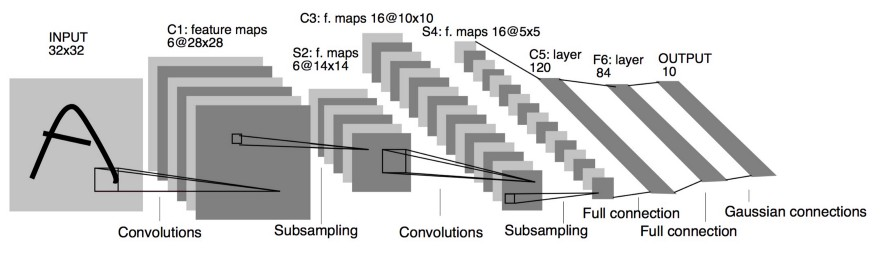
\includegraphics[scale=0.4]{figures/chapter1/lenet.jpg}
  \caption{Graphical representation of the LeNet architecture proposed by \citet{lecun1998gradient}}
  \label{figure:lenet_network}
\end{figure}

A perfect example of neural networks with a specific architecture are \emph{Convolutional Neural Networks} (CNN)~\cite{lecun1998gradient,krizhevsky2012imagenet,He_2016_CVPR,tan2019efficientnet} which consists of neural networks with specific structured linear transformations. 
The structured linear transform used in convolutional layers is the discrete convolution which consists of a kernel sliding over the image and acting as a filter.
% A perfect example of such efficient linear operation is the discrete convolution which consists of a kernel sliding over the image and acting as a filter.
Let $\avec$ and $\bvec$ be two vectors indexed by the set $M = \{-m, -m+1, \dots, m-1, m\}$, the discrete convolution between the signals $\avec$ and $\bvec$ is given by: 
\begin{equation}
  (\avec \ast \bvec) \left[ n \right] \triangleq \sum_{m \in M} \avec\left[m\right] \cdot \bvec\left[n - m\right]
\end{equation}
The convolution operation has translation invariance characteristics \cite{zhang1990parallel} which is perfectly suited for image classification (objects can be at different positions in images).  
\citet{lecun1998gradient} was one of the first to successfully train a convolutional neural network, achieving state-of-the-art performance on the MNIST dataset.
Convolution neural networks achieve such a great result for two main reasons:
first, CNNs are similar to the connectivity pattern of neurons in the visual cortex of the human brain. 
Secondly, CNNs are very efficient due to the sharing of parameters. 
While a classical linear operation with dense matrix has $n \times n$ parameters, a convolution only has $k \times k$ parameters where $k$ is the kernel size and is usually small (\eg 3 or 5 for classical convolution layers use in neural networks).
This weight sharing reduces the number of weights with respect to the fully connected neural network. The LeNet architecture (see Figure~\ref{figure:lenet_network}) has only $6 \times 10^4$ parameters.  


Although, convolutional neural networks perform well on specific tasks, important questions remain on the architecture of neural networks. 
% Which structure is better suited for neural networks?
Can we use other types of structure for neural networks?  
Does the reduction of parameters reduce the performance of the network?


%%%%%%%%%%%%%%%%%%%%%%%%%%%%%%%%%%%%%%%%%%%%%%%%%%%%%%%%%%%%%%%%%%%%%%%%%%%%%%%
\subsection{Structure Given by the Learning Procedure}
\label{subsection:ch1-introducing_structured_into_the_learning_procedure}
%%%%%%%%%%%%%%%%%%%%%%%%%%%%%%%%%%%%%%%%%%%%%%%%%%%%%%%%%%%%%%%%%%%%%%%%%%%%%%%

Instead of constraining the architecture of the network, we can constrain the learning procedure in order to reduce to search space.
Consider the following hypothesis space $\mathcal{H} = \left\{ f_\Theta \ |\ \Theta = ( \Wmat_1, \cdots, \Wmat_p ) \right\}$ which define the set of neural networks with fixed architecture.
We can introduce a structure in the hypothesis space by setting:
\begin{equation}
  \mathcal{H} = \left\{ f_\Theta \ |\ \Theta = ( \Wmat_1, \cdots, \Wmat_p ) \ |\ R(\Theta) \right\} 
\end{equation}
where $R(\Theta)$ is a constrain on $\Theta$ called a regularizer.
One of the most common form of regularization consists of adjusting the weights during the learning procedure under the constraint to keep the magnitude of the weights small.
This regularization has been introduced by~\citet{tikhonov_arsenin_1977} and is commonly known as \emph{weight decay}.
With this constraint, the hypothesis space can be defined as follows:
\begin{equation}
  \mathcal{H_\epsilon} = \left\{ f_\Theta \ |\ \Theta = (\Wmat_1, \cdots, \Wmat_p) \ | \ \norm{\Wmat_i}_\mathrm{F} \leq \epsilon \right\} 
\end{equation}
For a convex loss function, the minimization of the empirical risk within the set $\mathcal{H}_\epsilon$ can be achieved with the minimization of
\begin{equation}
  E(f_\Theta, n, \lambda) = \frac{1}{n} \sum_{i = 1}^{n} L\left(f_\Theta(\xvec^{(i)}), y^{(i)} \right) + \lambda \sum_{i = 1}^{p} \norm{\Wmat_i}_\mathrm{F}
\end{equation}
where $\lambda$ is a Lagrange multiplier.

Defining a regularization strategy is still an open problem in supervised learning. Recent works have proposed different form of regularization.  











%
%
% The concept of \emph{supervised learning} which refers to the notion of learning the parameters of a specific function (neural network) that maps an input to an output based on example input-output pairs.
% For example, an image (input) associated with its content: label (output).
% The steps of the learning procedure are as follows. 
% First, a neural network is initialized with random weights.
% Then, the algorithm \emph{analyzed} the training dataset and \emph{adjust} the weights in order for the network to correctly map the input to the output. 
%
% Due to the important expressivity of neural networks and of the finite number of sample data point, the learning procedure can produce a learned neural network that fits to closely on the training dataset and fail to fit on unseen example.
% This phenomenon is called \emph{overfitting} and can significantly decrease the general performance of neural networks.
% In order to limit overfitting and improve the general performance of neural network, \citet{vapnik1992principles} have proposed to constraint the learning procedure by adding a regularization term.  



% Another method proposed by \cite{vapnik1992principles} is to constraint the learning procedure in order to improve the performance of neural networks. 
%
% Important questions remain on supervised learning algorithms:
% Which properties can we leverage from these structures to improve the training and performance of neural networks? 


% Overfitting is a modeling error that occurs when a function is too closely fit to a limited set of data points. Overfitting the model generally takes the form of making an overly complex model to explain idiosyncrasies in the data under study.


% The choice of the function used for supervised learning is an active area of research and will be part of the focus of this thesis.
% In this work, we study \emph{neural networks} which are a class of function widely used for unstructured datasets (image, sound, text).






%%%%%%%%%%%%%%%%%%%%%%%%%%%%%%%%%%%%%%%%%%%%%%%%%%%%%%%%%%%%%%%%%%%%%%%%%%%%%%%
\section{Main contributions and Outline of the Thesis}
\label{section:ch1-main_contributions_and_outline_of_the_thesis}
%%%%%%%%%%%%%%%%%%%%%%%%%%%%%%%%%%%%%%%%%%%%%%%%%%%%%%%%%%%%%%%%%%%%%%%%%%%%%%%

%%%%%%%%%%%%%%%%%%%%%%%%%%%%%%%%%%%%%%%%%%%%%%%%%%%%%%%%%%%%%%%%%%%%%%%%%%%%%%%
\subsection{Main Contributions}
\label{subsection:ch1-main_contributions}
%%%%%%%%%%%%%%%%%%%%%%%%%%%%%%%%%%%%%%%%%%%%%%%%%%%%%%%%%%%%%%%%%%%%%%%%%%%%%%%

In this thesis, we leverage the properties of \emph{structured matrices} for the problems mentioned in Section~\ref{subsection:ch1-introducing_structured_into_the_architecture_of_neural_networks} and \ref{subsection:ch1-introducing_structured_into_the_learning_procedure}. A $n \times n$ structure matrix can be represented with less than $n^2$ parameters, Figure~\ref{figure:example_structure_matrices} shows an example of structured matrices.
In addition to offering a more compact representation, the structure of certain matrices can be leveraged to obtain better algorithms for matrix-vector product leading in memory and computationally operations. 

\begin{figure}[ht]
   \centering
   \begin{subfigure}[t]{0.24\textwidth}
       \centering
       \begin{equation*}
	  \leftmatrix
	    a &   &   &   \\
	      & b &   &   \\
	      &   & c &   \\
	      &   &   & d
	  \rightmatrix
       \end{equation*}
       \caption*{diagonal}
   \end{subfigure}
   \hfill
   \begin{subfigure}[t]{0.24\textwidth}
       \centering
       \begin{equation*}
	  \leftmatrix
	    a & b & c & d \\
	    e & a & b & c \\
	    f & e & a & b \\
	    d & f & e & a
	  \rightmatrix
       \end{equation*}
       \caption*{Toeplitz}
   \end{subfigure}
   \hfill
   \begin{subfigure}[t]{0.24\textwidth}
       \centering
       \begin{equation*}
	  \leftmatrix
	    ae & af & ag & ah \\
	    be & bf & bg & bh \\
	    ce & cf & cg & ch \\
	    de & df & dg & dh
	  \rightmatrix
       \end{equation*}
       \caption*{Low Rank}
   \end{subfigure}
   \hfill
   \begin{subfigure}[t]{0.24\textwidth}
       \centering
       \begin{equation*}
	  \leftmatrix
	    a & a^2 & a^3 & a^4 \\
	    b & b^2 & b^3 & b^4 \\
	    c & c^2 & c^3 & c^4 \\
	    d & d^2 & d^3 & d^4
	  \rightmatrix
       \end{equation*}
       \caption*{Vandermonde}
   \end{subfigure}
  \caption{Examples of structured matrices.}
  \label{figure:example_structure_matrices}
\end{figure}

More specifically, we study the proprieties of structured matrices from the Toeplitz family to make two contributions presented below:

\paragraph{Contribution 1} (C1)
We use circulant matrices, which are a particular case of Toeplitz matrices, to devise a new compact architecture replacing Fully Connected Neural Networks.
More precisely, we study deep diagonal circulant neural networks, which are deep neural networks in which weight matrices are the product of diagonal and circulant ones.
Besides making a theoretical analysis of their expressivity, we introduce principled techniques for training these models: we devise an initialization scheme and propose a smart use of non-linearity functions in order to train deep diagonal circulant networks. 
Furthermore, we show that these networks outperform recently introduced deep networks with other types of structured layers.
We conduct a thorough experimental study to compare the performance of deep diagonal circulant networks with state-of-the-art models based on structured matrices and with dense models.
We show that our models achieve better accuracy than other structured approaches while requiring 2x fewer weights than the next best approach.
Finally, we train compact and accurate deep diagonal circulant networks on a real-world video classification dataset with over 3.8 million training examples. 

\paragraph{Contribution 2} (C2)
It is well known that a discrete convolution operation with a 2d kernel applied on a 2d signal is equivalent to a matrix multiplication with a doubly-block Toeplitz matrix~\cite{jain1989fundamentals} (see Appendix~\ref{xxx}). 
Based on this knowledge and by leveraging the theory of Toeplitz matrices, we introduce a new upper bound on the Lipschitz constant for convolutional layers that is both tight and easy to compute.
This bound allows us to tackle the problem of Lipschitz regularization of Convolutional Neural Networks which is established now established as a key property of modern deep learning with implications in training stability, generalization, robustness against adversarial examples, etc.

% we leverage the properties of doubly-block Toeplitz matrices to devised a new fast and efficient method to compute the Lipschitz constant of convolutional layers. 
%
% However, computing the exact value of the Lipschitz constant of a neural network is known to be NP-hard.
% Recent attempts from the literature introduce upper bounds to approximate this constant that are either efficient but loose or accurate but computationally expensive.
% In this work, Based on this result we devise an algorithm to train Lipschitz regularized Convolutional Neural Networks.
%
% The contributions of this Thesis are based on structured matrices from the Toeplitz family.
%
% More specifically, in Chapter~\ref{chapter:diagonal_circulant_neural_network}, In Chapter~\ref{chapter:lipschitz_bound}, we leverage the structure of convolutional layers to devise a new regularization scheme for neural networks. 


%%%%%%%%%%%%%%%%%%%%%%%%%%%%%%%%%%%%%%%%%%%%%%%%%%%%%%%%%%%%%%%%%%%%%%%%%%%%%%%
\subsection{Outline of the Thesis}
\label{subsection:ch1-outline_of_the_thesis}
%%%%%%%%%%%%%%%%%%%%%%%%%%%%%%%%%%%%%%%%%%%%%%%%%%%%%%%%%%%%%%%%%%%%%%%%%%%%%%%

\todo{update this paragraph at the end of the writing}

% The thesis is organized as follows. The first Chapter (Chapter~\ref{chapter:related_work}) is dedicated to enumerating state-of-the-art approaches on both contributions. In a first part, we review approaches on compact neural networks. In a second part, we review  
%
% Chapter~\ref{chapter:related_work} present a related work in two parts: first we review existing techniques for on building compact neural network architecture. Then, we present different techniques to constraint the learning procedure. 
%
% The following two chapters contains the main contributions of the Thesis.  
% Finally, Chapter~\ref{chapter:conclusion} provides concluding remarks and a discussion.


